\documentclass{report}
% Include all project wide packages here.
\usepackage{fullpage}
\usepackage[style=ieee]{biblatex}
\usepackage[dutch]{babel}

\renewcommand{\familydefault}{\sfdefault}

\setmainfont[Ligatures=TeX]{Myriad Pro}
\setmathfont{Asana Math}
\setmonofont{Lucida Console}

\usepackage{titlesec, blindtext, color}
\definecolor{gray75}{gray}{0.75}
\newcommand{\hsp}{\hspace{20pt}}
\titleformat{\chapter}[hang]{\Huge\bfseries}{\thechapter\hsp\textcolor{gray75}{|}\hsp}{0pt}{\Huge\bfseries}
\renewcommand{\familydefault}{\sfdefault}
\renewcommand{\arraystretch}{1.2}
\setlength\parindent{0pt}

%For code listings
\definecolor{black}{rgb}{0,0,0}
\definecolor{browntags}{rgb}{0.65,0.1,0.1}
\definecolor{bluestrings}{rgb}{0,0,1}
\definecolor{graycomments}{rgb}{0.4,0.4,0.4}
\definecolor{redkeywords}{rgb}{1,0,0}
\definecolor{bluekeywords}{rgb}{0.13,0.13,0.8}
\definecolor{greencomments}{rgb}{0,0.5,0}
\definecolor{redstrings}{rgb}{0.9,0,0}
\definecolor{purpleidentifiers}{rgb}{0.01,0,0.01}


\lstdefinestyle{csharp}{
language=[Sharp]C,
showspaces=false,
showtabs=false,
breaklines=true,
showstringspaces=false,
breakatwhitespace=true,
escapeinside={(*@}{@*)},
columns=fullflexible,
commentstyle=\color{greencomments},
keywordstyle=\color{bluekeywords}\bfseries,
stringstyle=\color{redstrings},
identifierstyle=\color{purpleidentifiers},
basicstyle=\ttfamily\small}

\lstdefinestyle{c}{
language=C,
showspaces=false,
showtabs=false,
breaklines=true,
showstringspaces=false,
breakatwhitespace=true,
escapeinside={(*@}{@*)},
columns=fullflexible,
commentstyle=\color{greencomments},
keywordstyle=\color{bluekeywords}\bfseries,
stringstyle=\color{bluestrings},
identifierstyle=\color{purpleidentifiers}
}

\lstdefinestyle{vhdl}{
language=VHDL,
showspaces=false,
showtabs=false,
breaklines=true,
showstringspaces=false,
breakatwhitespace=true,
escapeinside={(*@}{@*)},
columns=fullflexible,
commentstyle=\color{greencomments},
keywordstyle=\color{bluekeywords}\bfseries,
stringstyle=\color{redstrings},
identifierstyle=\color{purpleidentifiers}
}

\lstdefinestyle{xaml}{
language=XML,
showspaces=false,
showtabs=false,
breaklines=true,
showstringspaces=false,
breakatwhitespace=true,
escapeinside={(*@}{@*)},
columns=fullflexible,
commentstyle=\color{greencomments},
keywordstyle=\color{redkeywords},
stringstyle=\color{bluestrings},
tagstyle=\color{browntags},
morestring=[b]",
  morecomment=[s]{<?}{?>},
  morekeywords={xmlns,version,typex:AsyncRecords,x:Arguments,x:Boolean,x:Byte,x:Char,x:Class,x:ClassAttributes,x:ClassModifier,x:Code,x:ConnectionId,x:Decimal,x:Double,x:FactoryMethod,x:FieldModifier,x:Int16,x:Int32,x:Int64,x:Key,x:Members,x:Name,x:Object,x:Property,x:Shared,x:Single,x:String,x:Subclass,x:SynchronousMode,x:TimeSpan,x:TypeArguments,x:Uid,x:Uri,x:XData,Grid.Column,Grid.ColumnSpan,Click,ClipToBounds,Content,DropDownOpened,FontSize,Foreground,Header,Height,HorizontalAlignment,HorizontalContentAlignment,IsCancel,IsDefault,IsEnabled,IsSelected,Margin,MinHeight,MinWidth,Padding,SnapsToDevicePixels,Target,TextWrapping,Title,VerticalAlignment,VerticalContentAlignment,Width,WindowStartupLocation,Binding,Mode,OneWay,xmlns:x}
}

%defaults
\lstset{
basicstyle=\ttfamily\small,
extendedchars=false,
numbers=left,
numberstyle=\ttfamily\tiny,
stepnumber=1,
tabsize=4,
numbersep=5pt
}
\addbibresource{../../library/bibliography.bib}

\title{EPO-2: Mid-term Design Report - routevolger}
\author{Tijmen Witte}

\begin{document}

\chapter{Routevolger}
\label{ch:routevolger}

Als er naar het grid wordt gekeken in hoofdstuk \rev{ch:probleemstelling} kan men zien dat er meer bij komt kijken dan alleen het volgen van een lijn, zoals in het vorige hoofdstuk beschreven is.

Doordat er kruispunten aanwezig zijn, ontstaan er drie mogelijke wegen die de robot kan nemen.
Bij het volgen van de route moet de robot rekening houden met de kortste route en hier op inspelen.
Mochten er mijnen op de route liggen dan moet de robot op het moment dat hij deze herkend terugrijden, zodat de lichtsensoren weer voor het kruispunt zitten.
Is dit niet het geval dan slaat hij het kruispunt over, waardoor hij letterlijk de weg kwijt is.

\section{Eisen}
De robot moet een kruispunt kunnen herkennen en vervolgens de keuze kunnen maken welke weg hij ingaat.
Deze keuze is afhankelijk van de kortste route die de robot kan nemen.
Als de robot van startpunt 1 naar eindpunt 6 gaat, is het onlogisch om bij het eerste kruispunt naar links te gaan, aangezien de robot dan verder van het eindpunt wegrijdt.
Verder moet de robot achteruit kunnen rijden.

\section{Ontwerp}
Het ontwerp van de routevolger is een aanvulling op de code van de lijnvolger.
Zo moet er in de VHDL-code extra worden weergegeven wanneer de robot op een kruispunt staat.
Mocht de robot op een kruispunt staan dan geven de lichtsensoren de bit '000' door. Hierdoor weet de robot dat hij op een kruispunt staat.
Verder moet de robot bochten kunnen maken wat te maken heeft met de VHDL-code van de servo-motoren.

\section{Implementatie}
Onze implementatie van de lijnvolger is te vinden in bijlage \ref{ssec:controller.vhdl}.

\section{Test}
We hebben een eigen testveld gemaakt, waarop we de robot hebben kunnen testen.
Dit veld is te zien in afbeelding \ref{fig:testfield}.
Door de robot van punt $1_A$ naar punt $3_B$ te laten rijden, hebben we kunnen testen of de robot de kruispunten herkende en of hij de bochten in de juiste richting nam.
Nadat de mijnendetector was aangesloten, hebben we mijnen geplaatst op de middenstukken en konden we testen of de robot op het juiste moment terugreed als hij een mijn had gedetecteerd. Na het terugrijden zouden de lichtsensoren weer voor het kruispunt recht op de lijn moeten zitten.

\begin{figure}[H]
	\centering
	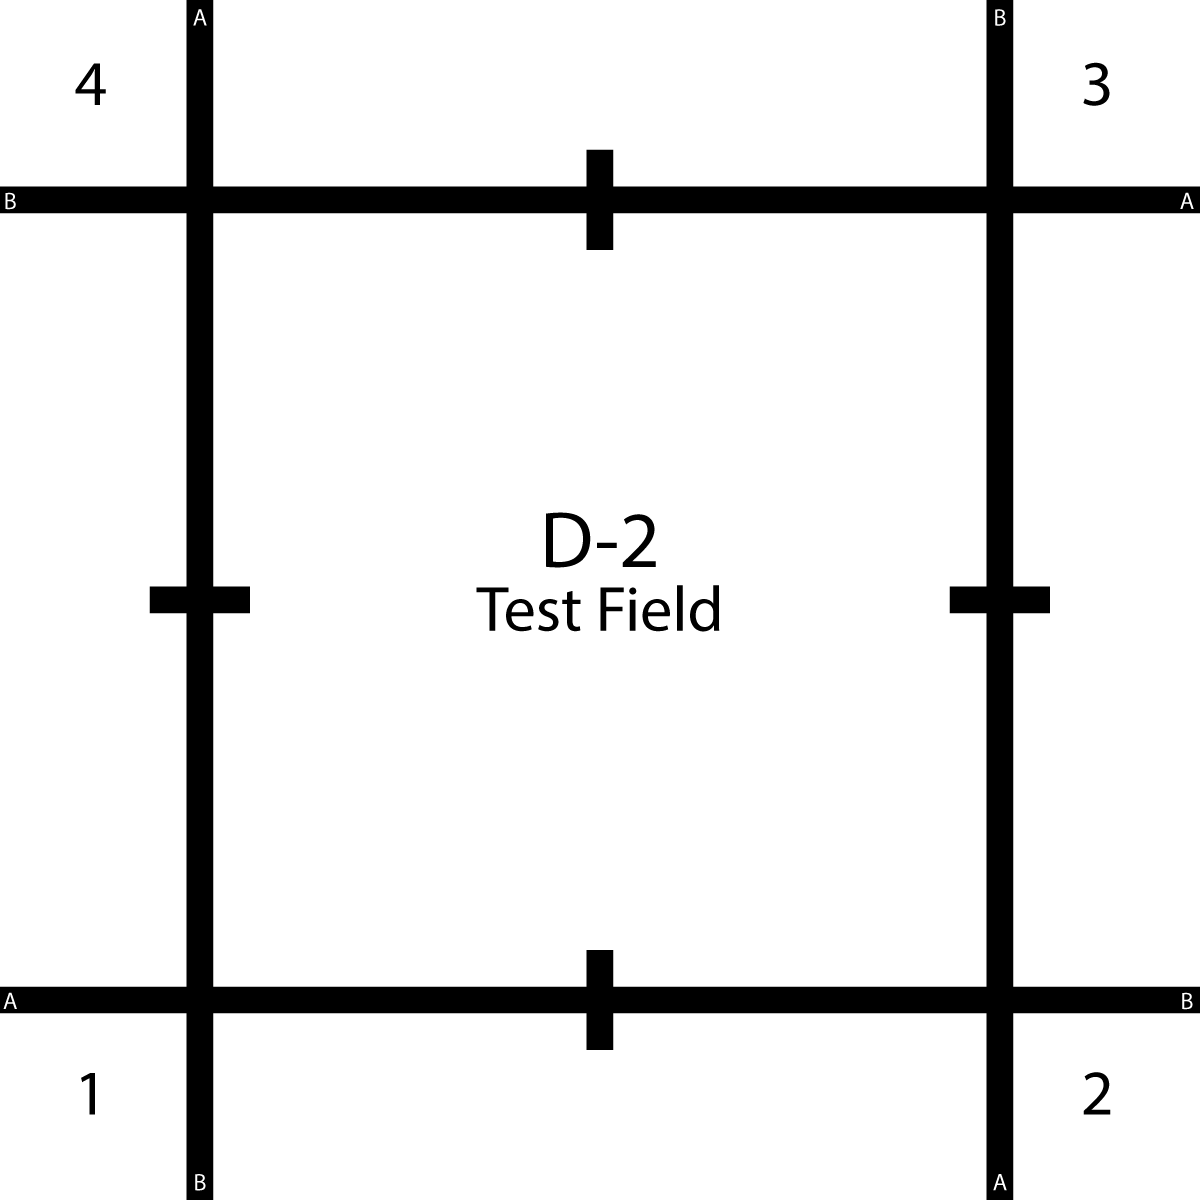
\includegraphics[width=0.5\textwidth]{d-2_test_field.png}
	\caption{Zelf gemaakt testveld voor EPO-2}
	\label{fig:testfield}
\end{figure}

\section{Discussie}


Bij het testen met het detecteren van de mijnen en het vervolgens laten terugrijden van de robot, kwamen we er achter dat de robot stopte nadat hij terug op het vorige kruispunt was. Dit was natuurlijk niet de bedoeling.
Door goed te kijken naar de VHDL-code, hebben we de fout kunnen vinden en deze weten te verhelpen.

%zijn we er achter gekomen dat de lichtsensoren meestal op het kruispunt terecht kwamen.
%Dit was natuurlijk niet de bedoeling.
%We hebben dit aangepast door de mijnendetector dichter bij het wiel te zetten, waardoor de mijn later werd gedetecteerd en bij het draaien van de robot, de lichtsensoren precies voor het kruispunt uitkwamen.
%Ook hebben we om dezelfde reden de lichtsensoren dichterbij het draaipunt van de robot geplaatst.

\end{document}